\chapter{Related Work} \label{chapter:related_work}

In the following chapter, we investigate the current state of research on 6D pose estimation. It starts with an excerpt of non-learning-based methods. We then present more recent, learning-based works with emphasis on active learning and fine-tuning of neural networks.

\section{Research on 6D Pose Estimation}

Pose estimation has become an increasingly interesting problem with the advent of robots in production and the area of virtual and augmented reality \cite{bb8}. Early research focused on manual feature extraction, divided into the major groups of sparse, dense and template-based approaches. Nowadays scientists often employ learning-based techniques which offer higher accuracy.

\subsection{Non-Learning-Based}

Before the major breakthrough of deep learning in 2012 \cite{alexnet}, handcrafted feature-based approaches were common for 6D pose estimation \cite{ylecun}. A lot of research matches sparse characteristics detected in the image against a database that contains the related pose information. The works of \cite{dglowe1, dwagner} use keypoints as the discriminative feature and offer good accuracy on well-textured objects. Unfortunately, precision declines for poor-textured or texture-less objects, because in those cases detectors are unable to find stable keypoints or any at all. The methods presented in \cite{gklein,dglowe2,charris} identify edges in the image and use different techniques to obtain an initial pose guess based on those edges. The resulting pose is retrieved iteratively refining the previous guess, by minimizing the distance of the projected and detected edges.
\nnewline
Template-based methods \cite{hinterstoisser1, hinterstoisser2, rioscabrera, csteger} use generated views of discrete viewopints on the object at different angles which are matched against the given image to retrieve the pose. This approach relies mainly on the shape of objects and thus works well for poor-textured or textureless objects \cite{pertsch}. To cover many objects and a large pose range, the number of templates of an object has to be increased though, which slows down prediction. Hashing the views to speed up the pose estimator reduces accuracy \cite{zhou}. Additionally, deformed or occluded objects decrease precision, as templates globally reason about the object's pose.
\nnewline
Some authors draw on multiple views to improve accuracy. Stereo cameras are used in \cite{kpauwels}. A second image from another angle implies depth information to a certain extend but involes the additional task of stereo matching. The availability of cheap depth sensors, like the Kinect, gave rise to algorithms making use of RGB-D images. Multiple approaches are possible when incorporating depth to retrieve an object's pose. Voting schemes were employed in \cite{bdrost, salasmoreno} and achieved good precision. First, a point in the image, potentially on the surface of the object, is selected and paired with all other scene points. This so-called point pair feature then votes for a possible pose, if the combination of their distance and respective normals are contained in the global sparse model description. The pose with the most votes is deemed to be the optimal one.

\subsection{Learning-Based}

Methods that learn information about objects - that is not explicitly modeled - started to outperform the previous techniques. There exist a vast literature for this task but we restrict our review to recent works that are most relevant to our approach.
\nnewline
Lai \etal use decision tress in \cite{klai}, which incorporate the semantic information of objects and their poses. Tom{\`{e}} \etal predict human poses from single RGB images in an end-to-end manner \cite{dtome}. The system developed in \cite{azeng} relies on multi-view images and depth information to retrieve an object's pose in a cluttered and occluded environment and scored the 3rd and 4th place in the Amazon Picking Challenge 2016 \cite{apc}. A prominent example of camera localization, which represents the problem of estimating the camera position in 3D space relative to the scene, is PoseNet \cite{posenet}. The underlying architecture of the employed neural network is based on GoogleNet, which was introduced in \cite{googlenet}. The CNN estimates the camera position directly without regression from a single image and is fast. In some indoor cases, PoseNet has an error as high as 50 centimeters, but our application demands high accuracy.

\paragraph{BB8.}

The recently developed BB8 \cite{bb8}, which is an abbreviation for the 8 corners of the bounding-boxes of objects, is the result of the work of Rad and Lepetit that operates on RGB-only images. Instead of regressing the pose of an object with object coordinates (see Section \ref{objectcoordinates}) like \cite{brachmann1}, they let a deep neural network estimate the object segmentations first (see Figure \ref{fig:bb8_segmentation}) and then predict the 2D locations of the 3D corners of the object's bounding box. An example of the corners can be seen in Figure \ref{fig:bb8}.
\nnewline
\begin{figure}[!tbp]
	\centering
	\begin{subfigure}[b]{0.45\textwidth}
		\centering
    	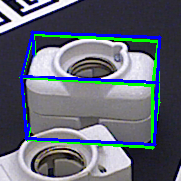
\includegraphics[width=0.45\linewidth]{bb8_prediction}
    	\caption{The corners of the object's bounding box.}
    	\label{fig:bb8}
	\end{subfigure}
	\hfill
	\begin{subfigure}[b]{0.45\textwidth}
		\centering
    	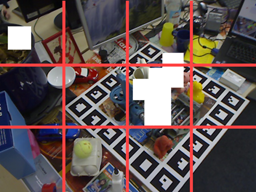
\includegraphics[width=0.45\linewidth]{bb8_segmentation}
    	\caption{The segmentation preceding the pose estimation.}
    	\label{fig:bb8_segmentation}
	\end{subfigure}
	\caption{Example images displaying the functioning of BB8. Images from \cite{bb8}.}
\end{figure} 
\noindent
Similar to \cite{brachmann1}, the object's position is not predicted directly either, but instead regressed by solving the perspective-n-point problem (PnP) of the correspondences of the corners of the object's bounding box and the projected locations of the corners in the image. The architecture of the first and second net is based on VGG \cite{vgg} respectively but with the last layer cut off and replaced by a fully connected layer which is fine-tuned. 
\nnewline
The first neural network, which segments the image, helps estimating the pose of the object in a way that the second network positions its window at the center of the segmentation and estimates the 2D locations of the 3D corners of the object's bounding box. The network reasons globally about the object by not moving the window during training and prediction. The authors argue that patch-based pose estimators are typically very noisy, and hence require a robust optimization scheme, like RANSAC. 
\nnewline
Unfortunately, BB8's take on pose estimation fails on symmetric objects, when implemented directly as described above. To address this problem, the authors first estimate the rotational angle of the object using a neural net, and mirror the image if necessary. This way, a CNN can be trained only on a certain range of the angle of the pose.
\nnewline
The proposed method offers good performance and can compete with and partly surpasses state-of-the-art research. Yet, object coordinates provide high accuracy too. Furthermore, we assume that the often merely partial visibility of the surgical instruments calls for a non-global reasoning design. Thus, BB8 is not followed any further in this work.

\paragraph{SSD-6D.}

The system presented in \cite{ssd-6d} is based on the Single-Shot Multibox Detector (SSD) \cite{ssd}. Their take on 6D pose estimation is especially alluring, as the authors train the network exclusively on synthetic data. A positive outcome would imply that the lack of already annotated datasets for 6D pose estimation could be overcome by generating data for network training. 
\nnewline
\begin{figure}[!tbp]
	\centering
	\begin{subfigure}[b]{0.3\textwidth}
		\centering
    	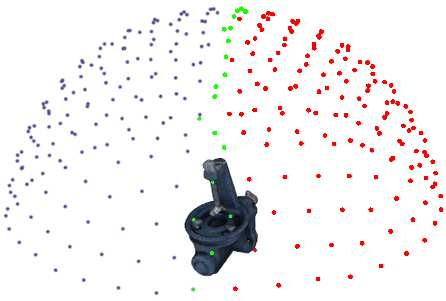
\includegraphics[width=\linewidth]{ssd_6d_sphere}
    	\caption{An exampe of a discrete distribution of viewpoints on an object.}
    	\label{fig:ssd6d_viewpoints}
	\end{subfigure}
	\hfill
	\begin{subfigure}[b]{0.6\textwidth}
		\centering
    	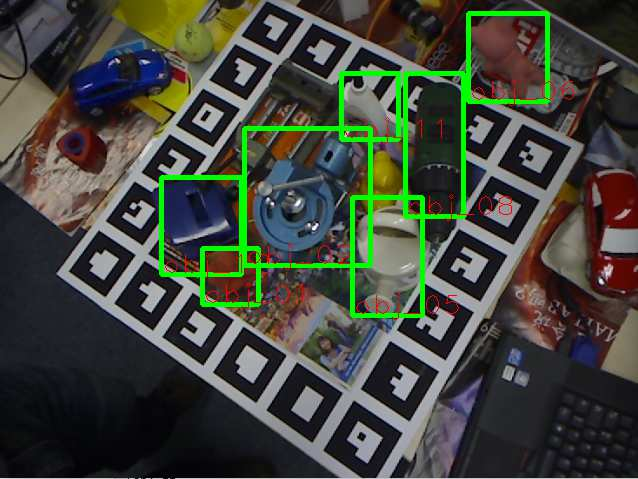
\includegraphics[width=0.45\linewidth]{ssd_6d_bb}
    	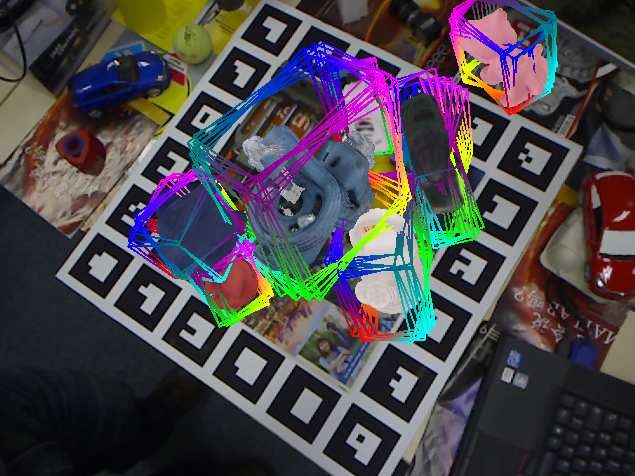
\includegraphics[width=0.45\linewidth]{ssd_6d_pose}
    	\caption{Left image: An example for bounding boxes found by the SSD-6D network. Right image: The most confident views and rotations for those boxes.}
    	\label{fig:ssd6d_detection}
	\end{subfigure}
	\caption{Example images displaying the functioning of SSD-6D. Images from \cite{ssd-6d}}
\end{figure}
The SSD-inspired network architecture produces feature maps of the input images, that are convolved to predict the class and 2D bounding box (see Figure \ref{fig:ssd6d_detection} left) of objects in the scene. The network also estimates the probability of a discrete viewpoint on the object. Those viewpoints are sampled equidistantly alongside a predefined step size (see Figure \ref{fig:ssd6d_viewpoints}). The pose is calculated taking into account the class, bounding box, viewpoint and a guess on the in-plane rotation of the object. The network is trained entirely on images from the MS COCO dataset \cite{mscoco}. The objects that are to be detected are rendered into them with arbitrary translations and rotations. For each transformation, the network is given the closest discrete viewpoint, in-plane rotation and the tightest bounding box as a regression target.
\nnewline
The author's reasoning, that their approach on pose estimation is a more natural one than pose regression. This stands to reason, as a human learns what an object looks like by viewing it from different angles. Nevertheless, the network produces rather inaccurate initial results.  To remedy this drawback, an optimization scheme extracts 3D contour points from the rendered hypothesis and minimizes the distance to the detected 2 locations of the points on the image. 
\nnewline
The neural network alone performs less well compared to \cite{brachmann1} or \cite{bb8}. The optimization process could also be applied to the two mentioned works. Hence it is not investigated further. 

\paragraph{Kurmann \etal}

The work of \cite{kurmann} estimates poses of surgical instruments in minimally invasive surgery. Similarly to object coordinate regression, Kurmann \etal develop a system that produces probabilities of the presence of an object but not in a dense way but instead only for the joints of the tools. Their design draws on a scene model which holds how many tools can be visible at most, what tools are currently visible and what parts of those tools.
\nnewline 
The authors of that paper argue that the common two-stage pipeline for 6D pose estimation, that consists of object detection and then pose estimation, results in a more complicated design, and criticize that a sliding window approach might miss very small or very large instruments, i.e. advocate a global reasoning design.
\nnewline
The architecture of the employed network is based on the U-Net developed by the authors of \cite{oronneberger}, and trained by optimizing the cross-entropy derived from the scene model described earlier. The network architecture of U-Net is extended by a fully connected layer that is trained to predict the probabilities of the instruments.
\nnewline
The results of the design look promising and run time per image is around $100 ms$, enabling it to be deployed as a real-time solution. Conversely, mainly literature of the biomedical imaging was considered and compared, disregarding research work in other areas on pose estimation.

\subsection{Learning-Based: Object Coordinate Regression}

There exists interesting work achieving high accuracy by using object coordinate regresseion. The idea is based on \cite{tsharp} and \cite{firstcoordinateregression}. The first used it to estimate the pose of a human body, the latter to regress the cameras position in a scene retrieved from a single RGB-D image.
\nnewline
Brachmann \etal achieved record-breaking results in \cite{brachmann1} for texture-less objects and good performance in general. The authors based their work on forests instead of trees to regress the object's pose. The forests are trained to jointly predict the probability of object instances as well as the object coordinate probability for a given pixel. The output of the forest is processed in an energy function that imposes an energy minimization problem to regress the object's pose. A RANSAC-like scheme then iteratively refines the pose.
\nnewline
In \cite{brachmann2}, Brachmann \etal adjusted their pipeline from \cite{brachmann1} to work with RGB-only images. To reduce uncertainty in the object instance and coordinate predictions they incorporate an auto-context framework and marginalize the object coordinates over the depth information to cope with the missing fourth channel. The presented system outperforms Brachmann \etal's previous work but is still based on forests. 
\nnewline
Krull \etal elaborated \cite{brachmann1} by replacing the energy function by a CNN \cite{akrull}. They were able to further improve the performance and transfer object coordinate regression to modern deep neural networks. The system called PoseAgent fuses regression forests and CNNs \cite{poseagent}. The regression forest outputs pose hypotheses that the CNN then refines. Krull \etal are able to achieve state-of-the-art results and improve resource utilization. Although \cite{trees-vs-cnn} finds, that random forests partly offer a slightly superior performance, neural networks can compete and are therefore the focus of this work.

\paragraph{Pertsch.}

Although \cite{pertsch} also works with RGB-D images, we present his work here as the author proposes an easy extension to adapt the entire process to RGB-only images and presents promising results. The work by Pertsch is based on \cite{brachmann1}, i.e. uses object coordinates  (see section \ref{objectcoordinates}), but replaces the random forest with a CNN. The developed pose estimation pipeline relies on three steps. The first one segments the image, the second regresses the object coordinates, and the last one evaluates pose hypotheses. 
\nnewline
We don't to go into detail into the first operation of the pipeline as our training and test data already includes segmentations and we can hence omit it completely. The second stage consists of a multilayer CNN-architecture to predict the object coordinates. The architecture consists of an encoder-decoder multilayer network. Inspired by \cite{oronneberger}, the author assimilates skip-layer connections. The network computes object coordinates for each pixel of the previously computed segmentation. Pertsch employs a RANSAC-scheme to improve the quality of the predicted final pose. Two different methods to retrieve the pose are presented in the work, one relying on the energy function introduced in \cite{brachmann1} but in an altered version, and one procedure solely drawing on RGB information without the additional depth of a sensor. The latter, which is more relevant for us as we do not have any depth readings, is based on the earlier presented \cite{brachmann2}. 
\nnewline
Instead of penalizing depth divergences of the rendered depth from the estimated pose and the sensor readings, the number of pixels whose reprojection error is greater than a certain threshold is minimized iteratively by the RANSAC algorithm. This allows for the RGB-only extension that the author suggests but does not elaborate in detail. Without depth the pose regression becomse a PnP problem, that can be solved by a PnP solver which takes at  four 3D-2D point correspondences as input. We pursue a similar approach in our work which differs in architecture of the network, the steps of the pipeline and the input data. But the general ideas of \cite{pertsch} and especially \cite{brachmann1} are adopted and further complemented with current research and active and incremental learning.

\section{Research on Active and Online Learning}

Online learning considers how to incorporate new available data into a trained model or neural network. Active learning is the field of selecting data that a human should annotate manually, because the model does not perform well on it. The literature survey \cite{activesurvey} gives an overview over methods developed before 2011. Wang and Shang, the authors of \cite{dwang}, might be among the first to incorporate active learning into deep learning though, according to \cite{zhou}. In \cite{hyperspectral}, Al Rahhal \etal apply a similar idea to hyperspectral image classification, a task that shares the foibles to be tedious and time-consuming with biomedical image annotation. The authors developed an active selection paradigm to electrocardiogram classification. 

\paragraph{Zhou \etal}

In \cite{zhou}, Zhou \etal describe a novel process of actively demanding data to be annotated to improve the network quality and apply the newly available data in an incremental manner. They focus on this area because annotating biomedical images is still a time-consuming task that requires a lot of expertise and skill.
\nnewline
Opposed to retraining from scratch, the network is fine-tuned by an incremental tuning algorithm. According to the authors, researchers have shown that this offers superior performance. In contrast to our task, the authors want to achieve improvements on image classification and frame detection, but work on biomedical images nonetheless.
\nnewline
\begin{figure}[!tbp]
	\centering
    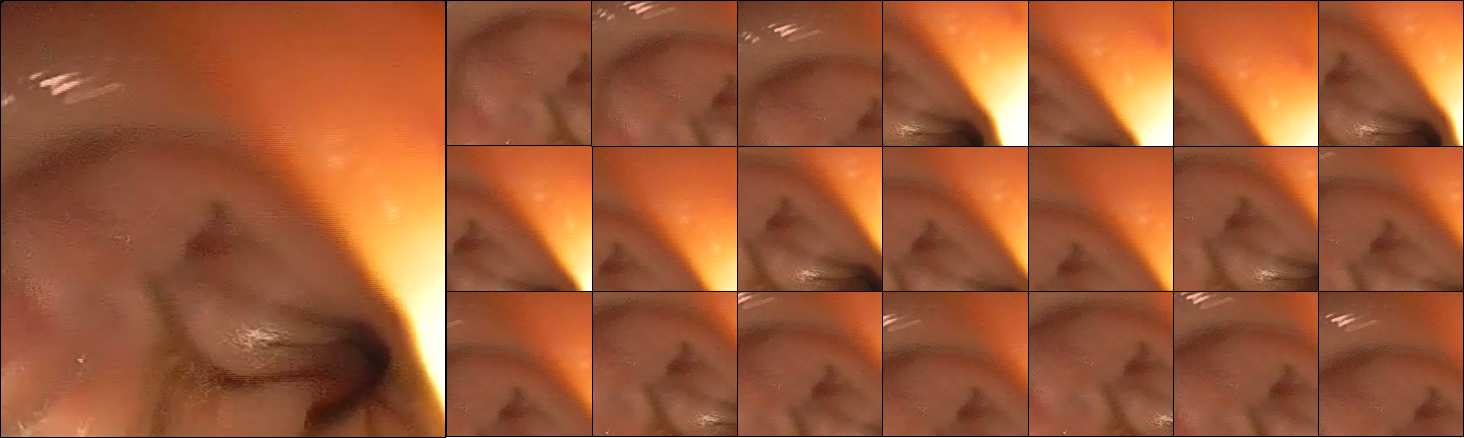
\includegraphics[width=0.7\linewidth]{fine_tuning}
	\caption{A candidate (left) and the patches generated sharing the same label. Images from \cite{zhou}.}
	\label{fig:zhou}
\end{figure}
Computer-aided-diagnosis (CAD) systems usually provide a candidate generator, which can quickly produce candidates, including true and false positives, to train with. Through data augmentation the learner can be made more robust to unforeseen situations. For this, numerous patches sharing the same label are generated from the candidate, as can be seen in Figure \ref{fig:zhou}, an presented to the classifier. 
\nnewline
The active selection process of candidates requires a measure of the worthiness of a candidate. To achieve this, the entropy and diversity of patches are calculated using the network's predictions for the patches of a candidate. Entropy is the negative log-likelihood of the network's prediction, whereas diversity captures how much patches of a candidate contradict, as they should all share the same label. Candidates with contradicting patches or low entropy can be selected for manual annotation.
\nnewline
The procedure quickly improves the neural network's accuracy. Learning from scratch or random selection of next candidates are quickly  outperformed, as only around 20\% of manually annotated candidates are necessary to reach the same error rate with the presented procedure.
\nnewline
In our case, data augmentation is possible, as we can render synthetic images, but the unnatural lightning and shadowing might decrease the accuracy of the design. The question of how to find  a worthiness measure arises too, as we can't directly tell how sure a network is when predicting a pose. But it provides a good direction of how to approach active learning.

\paragraph{Liu \& Ferrari.}

\begin{figure}[!tbp]
	\centering
    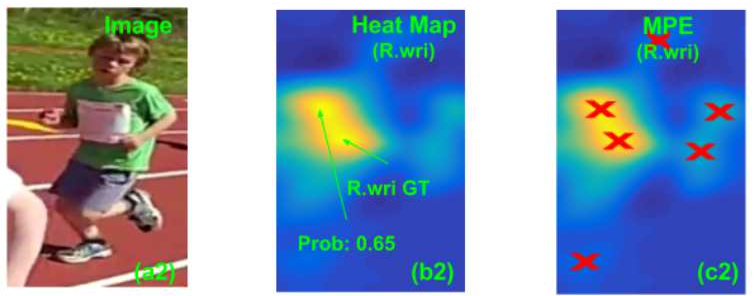
\includegraphics[width=0.6\linewidth]{human_pose_heatmap}
    \caption{An image of a human body, the corresponding heatmap as well as the result of the Multiple Peak Entropy (MPE). Images from \cite{humanpose}.}
    \label{fig:humanpose}
\end{figure}
In \cite{humanpose}, Liu and Ferrari describe new strategy for active learning for human pose estimation, a time-consuming task to produce groundtruth annotations for. Their key contributions consist of an uncertainty estimator for the joint predictions produced by a convolutional pose machine (CPM), and an annotation interface that reduces the time needed by a human annotator to click joints. The predictions by the CPM are heatmaps, with high temperature resembling the most probable position of the joints (the input image can be seen Figure \ref{fig:humanpose}(a2), the heatmap in \ref{fig:humanpose}(b2)).
\nnewline
The active learning scheme incorporates influence and uncertainty cues. Influence cues consider images that are similar to other unlabeled images could propagate information. The uncertainty cues are measured by the uncertainty estimator. The estimator focuses on uncertain predictions, i.e. predictions with multiple weak peaks (multiple peak entropy) (see Figure \ref{fig:humanpose} (c2)). The final selection process then takes both cues into account when requesting an image to be manually annotated.
\nnewline
In addition, an interface is proposed that reduces the annotation time significantly. The system predicts a pose and segments the image around joints. The user can then right click anywhere in the segmentation to accept the estimated joint location or manually select it.
\nnewline
The results of \cite{humanpose} look auspicious, as a reduction in annotation time can be achieved through the interface and the selection process. Regrettably, it cannot be directly applied to our problem, as we need a problem-specific certainty estimator. But the idea of requesting similar images to be annotated might yield a performance gain, and similarly to the presented interface we present the user with an initial probable pose, too, to make only small corrections necessary.